\selectlanguage{italian}%

\section{Soluzione}


\subsection{Schematici}

\begin{figure}[H]
	\centering
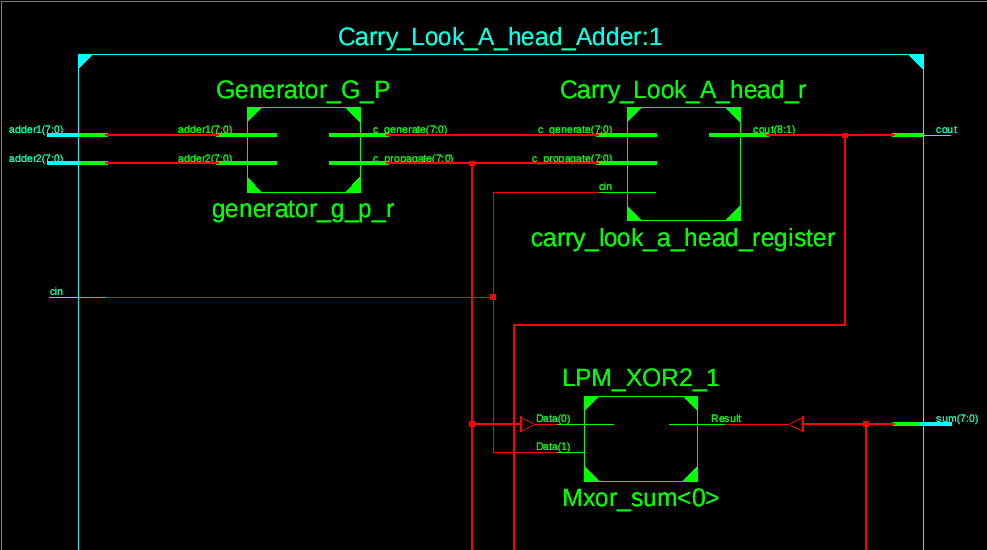
\includegraphics[scale=0.5]{esercizio09/images/carry_look_a_head_adder.png}
	\caption{Carry Look a Head}
\end{figure}

L' addizionatore � costituito, da una rete che permette di calcolare
i riporti generati e propagati, questi poi vengono propagati ad una
rete Carry Look A Head che contemporaneamente combina i riporti ricevuti,
altrimenti ci si riconducerebbe al caso Ripple Carry, dopodich� il
riporto generato dalla rete Carry Look A Head viene messo in ingresso
ad un XOR insieme al ritardo propagato, calcolato precedentemente.

\begin{table}[H]
\noindent\begin{minipage}[t]{1\columnwidth}%
\begin{tabular}{|c|c|c|c|}
\hline 
Numero di bit operandi & Numero di slice & Numero di four LUT & Tempo di calcolo\tabularnewline
\hline 
\hline 
4 & 6 & 8 & 7,190 ps\tabularnewline
\hline 
8 & 12 & 19 & 7,444 ps\tabularnewline
\hline 
16 & 24 & 32 & 9,006 ps\tabularnewline
\hline 
32 & 48 & 64 & 9,139 ps\tabularnewline
\hline 
\end{tabular}%
\end{minipage}
\end{table}

Secondo le formule dell' area e del ritardo, l' area � pari a $(n^{2}+9n)/2$
volte(dove $n$ indica il numero di porte logiche) , ed 5$/delta$,
ma se confrontiamo i risultati con quelli ottenuti sintetizzando il
Ripple Carry Adder \ref{Dati ripple carry}, possiamo osservare che
trascurando il caso 8 bit,  l' area occupata � pressoch� la stessa,
ma i tempi di calcolo sono sensibilmente minore, aiutando ad affermare
con certezza che sulla nostra FPGA tale soluzione risulta migliore.

\subsection{Codice}

\href{run:progetti/Carry_Look_A-head_Adder_with_test/Carry_Look_A-head_Adder.xise}{Carry Look A Head ISE}

\subsubsection{Carry Look A Head}

\lstinputlisting [language=VHDL,caption={Definizione del Carry Look a Head},firstline=32] {progetti/Carry_Look_A-head_Adder_with_test/Carry_Look_A_head_r.vhd}

Del Carry Look a Head ne viene generato uno di una dimensione pari
al numero di riporti propagati e generati da gestire.\selectlanguage{italian}%

